% ************************** Thesis Abstract *****************************
% Use `abstract' as an option in the document class to print only the titlepage and the abstract.
\chapter{Introduction}
\subsection{Motivation}

Tuning hyperparameters is considered a computationally intensive and tedious task, be it for neural networks, or complex physical instruments such as free electron lasers.
Users for such applications could benefit from a 'one-click-search' feature, which would find optimal parameters in as few function evaluations as possible.
This project aims to find such an algorithm which is both efficient and holds certain convergence guarantees.
We focus our efforts on Bayesian Optimization (BO) and revise techniques for high-dimensional BO. \\

\subsection{Background}

In Bayesian Optimization, we want to use a Gaussian Process to find an optimal parameter setting $\mathbf{x^*}$ that maximizes a given utility function $f$.
We assume the response surface to be Lipschitz-continuous. \\

Assume we have observations $ \mathcal{Y} = \{ y^{(1)}, \ldots, y^{(N)} \}$, each evaluated at a point $ \mathcal{X} = \{  \mathbf{x}^{(1)}, \ldots, \mathbf{x}^{(N)} \}$.
The relationship between the observations $y$ and individual parameter settings $\mathbf{x}$ is $y = f \left( \mathbf{x} \right) + \epsilon$ where $\epsilon \sim  \mathcal{N} \left( 0, \sigma^2_n \right)$. Any quantity to be predicted has a subscript-star (e.g. $y_*$ is the function evaluation we want to predict).\\

In it's simplest form, a Gaussian Process is described by the following equation:

\begin{equation}
\begin{pmatrix} y \\
y_* \end{pmatrix} \sim N\Biggl(\mu,\begin{pmatrix} K & K^T_*\\
 K_* & K_{**} \end{pmatrix}\Biggr),
\end{equation}

Where $\mu$ is a mean function, $K = \text{kernel}(\mathbf{X}, \mathbf{X})$, $K_* = \text{kernel}(\mathbf{x_*}, \mathbf{X})$ and $K_{**} = \text{kernel}(\mathbf{x_*}, \mathbf{x_*})$.
We predict any new point $y_*$, (given all previously sampled points $y$) by estimating the probability $ p(y_*|y) \sim N(K_*K^{-1}y,K_{**}-K_*K^{-1}K'_*) $

This, in turn, can be used to build an acquisition function. 
This acquisition function describes where to best sample points next.
Some popular acquisition functions include GP-UCB, Most probable improvement (MPI) and Expected Improvement (EI).
The choice of the acquisition function has great influence on the performance of the optimization procedure.\\

We will talk about the problems and possible solutions for the task at hand in the next section.

\subsection{Scope of the Project}

Bayesian optimization suffers from the curse of dimensionality. 
The goal of this project is to arrive at a solution that resolves the curse of dimensionality for the specific task with regards to Bayesian optimization.
This project includes, but is not limited to the following methods.\\

\begin{enumerate}
\item \cite{Tripathy}
Assume $f(x) \approx g( \mathbf{W}^T x)$ where $ \mathbf{W} \in \mathbb{R}^{D \times d} $ and $D >> d$.
We assume that $ \mathbf{W} $ is orthogonal as proposed in \cite{Tripathy}.

The algorithm does not require gradient-information (thus, easier to implement, and robust to noise).
The standard-deviation, kernel parameters and  $ \mathbf{W} $ can be found iteratively.
First, we fix $ \mathbf{W} $ and optimize over the standard-deviation, kernel parameters.
Then we fix the standard-deviation, kernel parameters. and optimize over $ \mathbf{W} $.
We repeat this procedure until the change of the log-likelihood between iterations is below some $ \epsilon_l $.

\item \cite{Rolland}
Assume $f(x) = f^{(1)}( x^{(1)} )  + f^{(2)}( x^{(2)} ) + \ldots + f^{(M)}( x^{(M)} )$ where $ x^{(i)} \in \mathcal{X}^{(i)} \subseteq \mathcal{X}$, i.e. each function component  $f^{(i)}$ takes some lower-dimensional subspace as the input.
The lower-dimensional subspaces may overlap.
The mean and covariance of $f(x)$ is then the sum of the individual component's means and covariances.

An additive decomposition (as described above) can be represented by a dependency graph. The dependency graph is built by joining variables $i$ and $j$ with an edge whenever they appear together within some set $x(k)$. 

The goal is to maximize an acquisition function $ \phi_t(x) = \sum_{i=1}^M \phi_t^{(i)} ( x^{(i)} )$. 
This maximization is achieved by maximizing the probability of Markov Random Fields within the graph.
A junction tree is created from the graph, which is then used to find the global maximum of the acquisition function.

The dependencies between the variable-subsets are represented through a graph, which can be learned through Gibbs sampling.
This, in turn, is used to create a kernel for the GP.

% TODO: cite rembo!
\item \cite{Wang}
A function $f : \mathbf{R}^D \rightarrow \mathbf{R}$ is said to have effective dimensionality $d_e$ (where $d_e < D$), if there exists a linear subspace $\mathcal{T}$ of dimension $d_e$ such that for all $ x_\top \in \mathcal{T} \subset \mathbf{R}^D $ and $x_\perp \in \mathcal{T_\perp} \subset \mathbf{R}^D $, we have $ f(x) = f(x_\top +x_\perp ) = f(x_\top)$.
$\mathcal{T^\perp}$ is the orthogonal complement of $\mathcal{T}$.

Assume $ f : \mathbf{R}^D \rightarrow \mathbf{R} $ has effective dimensionality $d_e$.
Given a random matrix $ \mathbf{A} \in \mathbf{R}^{D \times d} $ (where $d \geq d_e$) with independent entries sampled fom $ \mathcal{N}(0, 1) $.
For any $ x \in \mathbf{R}^D $, there exists a $y \in \mathbf{R}^d $ such that $ f(x) = f(\mathbf{A} y ) $.
We now only need to optimize over all possible $y \in \mathbf{R}^d$, instead of all possible $x \in \mathbf{R}^D $.


\begin{figure}[h]
\centering
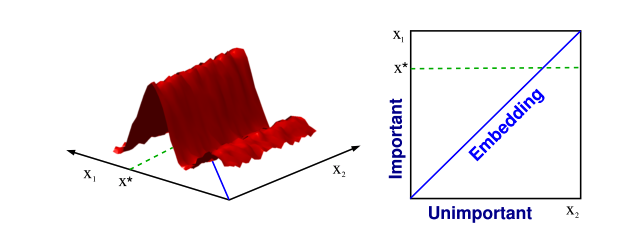
\includegraphics[width=0.5\textwidth]{./../src/Embedding_optimization.png}
\caption{ This function in D=2 dimesions only has d=1 effective dimension. Hence, the 1-dimensional embedding includes the 2-dimensional function’s optimizer. It is more efficient to search for the optimum along the 1-dimensional random embedding than in the original 2-dimensional space}
\end{figure}

\end{enumerate}

If for some reason, finding an active subspace or an effective lower dimension is not possible, we are open to adapt the procedure of optimization.
